
% ######################################################################### %
% ------------------------------------------------------------------------- %
%                   Anisotropy in Neural Connectivity
% ------------------------------------------------------------------------- %
% ######################################################################### %


\section{Anisotropy in Neural Connectivity}
\label{sec:biol_anisotropy}

Neurogeometry\index{neuro geometry} addresses the problem of inferring
synaptic connectivity from the geometric shapes of axon and
dendrites. A fundamental concept in this field is that of a
\textit{potential synapse}\index{potential synapse}
\parencite{Stepanyants2002}. Defined as the potential axonal-dendritic
connection of two neurons, present whenever the axon of one neuron is
within a spatial distance $s$ of the dendrite of the other, it is a
necessary, although not sufficient, condition for the formation of a
synaptic connection (\autoref{fig:potential_synapse}). The existence
of such close appositions solely depends on dendritic and axonal
anatomy; identification of defining morphological characteristics in
both axon and dendrite would therefore allow for a model of local
network connectivity, assuming for example that a certain ratio $r$ of
potential synapses turn into active contacts independently. It is the
hope that such a model, motivated from the geometry of a neuron's
functional compartments, not only displays inherent patterns of
connectivity similar to what has been observed in biological networks,
but also proofs itself as a testing ground for how this connectivity
may affect network dynamics.

\vspace{-0.21cm}
\definecolor{lightgray}{rgb}{0.88, 0.88, 0.88}
\begin{center}
 \setlength{\fboxrule}{0pt}
 \fcolorbox{black}{lightgray}{
   \begin{minipage}[c]{0.90\textwidth}

     \vspace{0.1cm}
     \setlength{\intextsep}{0pt}%
     \setlength{\columnsep}{8pt}%
     \begin{wrapfigure}{r}{0.65\textwidth}
       \captionsetup{labelformat=empty,labelsep=none}
       \centering
       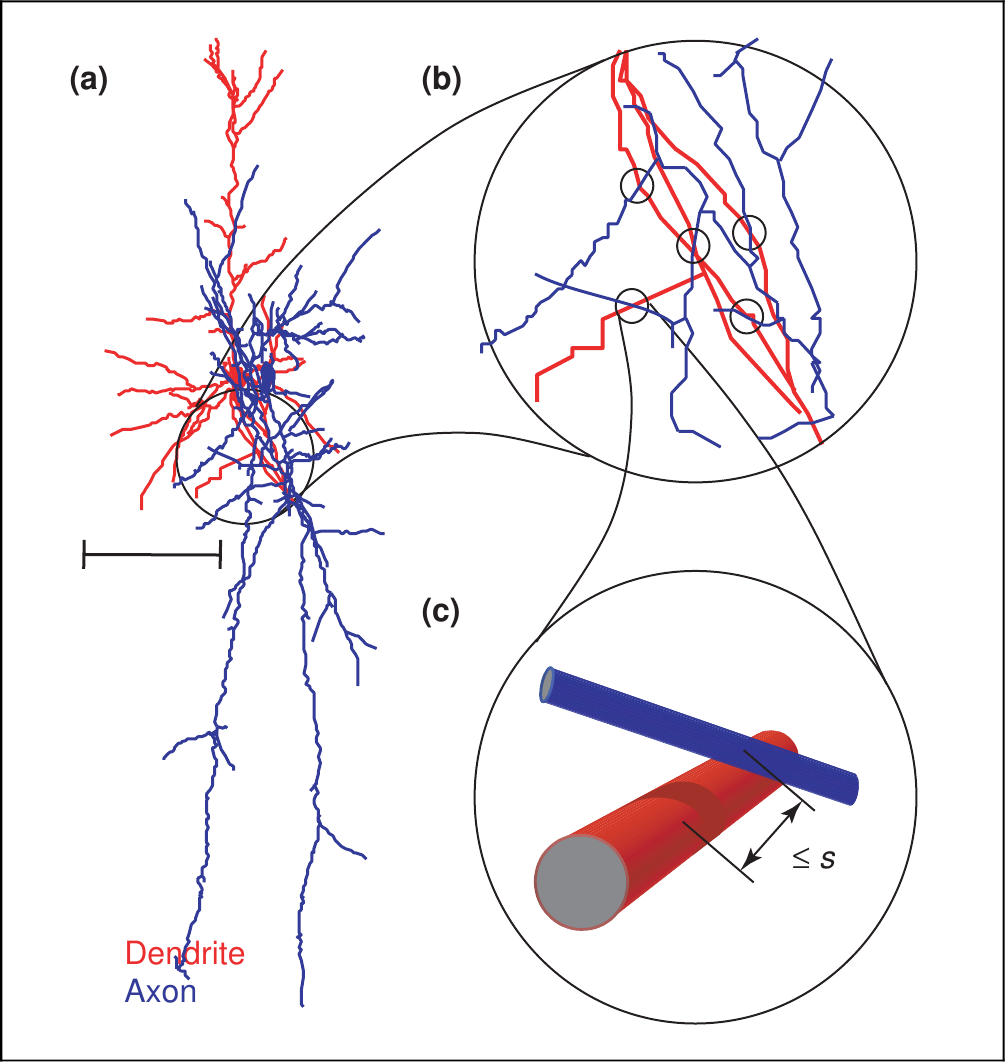
\includegraphics[width=\linewidth]{img/potential_synapse2.png}
       \vspace{-35pt}
       \caption{}
       \label{fig:potential_synapse}
     \end{wrapfigure}

     \footnotesize \textbf{Potential Synapse} 
     \smallskip

     Close ap\-positions be\-tween den\-drite and axon
     are a necessary condition for the formation of a synapse. \textbf{(a)}
     3-D reconstructions of a py\-ra\-mi\-dal cell den\-drite in red, axon of a
     regular spiking non-pyramidal cell in blue. \textbf{(b)-(c)}
     Overlapping arbors allow for several potential synapses whenever
     dendrite and axon are within a spatial distance $\leq s$. Values for
     $s$ depend on the type of synapse, typically between
     0.4-\SI{2}{\micro\meter}. Scale bar: \SI{100}{\micro\meter},
     \SI{30}{\micro\meter}, \SI{3}{\micro\meter} in (a),(b),(c)
     respectively. Image from \textcite{Stepanyants2005}. \hfill \textbf{4.1}

     \vspace{0.1cm}
   \end{minipage}}
\end{center}
%\vspace{-0.12cm}


Finding stereotypical anatomical characteristics however is difficult,
as axonal morphology is, in general, highly diverse
%------------------------------------------------
\marginpar{high variability in axonal morphology} 
%------------------------------------------------ 
\parencite{Debanne2004}. Across different species,
distinct regions in the central nervous system and different neuron
types, axons display a wide variety of shapes characterized by
morphometric parameters such as total length, branching complexity and
axonal extent \parencite{Ropireddy2011}. Typical examples of distinct
morphology include the T-shaped axons of cerebellar granule cells
branching only at a singular point \parencite{Cajal1911}, and axons of hippocampal CA3
pyramidal cells, which, in stark contrast, may feature up to 40
branches resulting in a total length of axon collaterals of up to
\SI{12}{\milli\meter} \parencite{Ishizuka1990}.

It is therefore imperative to confine this analysis to a specific
brain region and neuron type. In this study, we set the focus on
circuits of pyramidal cells in the mammalian cortex.
%?? Cortex does this
%?? Cortex is this well studied
%?? Here we go
More specifically, local circuits of thick tufted layer V
pyramidal neurons in the rat's somatsosensory cortex have been the
target of advanced
experimentation \parencite{Song2005,Perin2011,Romand2011, Ramaswamy2012}, and will
serve as a benchmark for results in neural morphology and network
connectivity in this report.


\begin{figure}[!htbp]
  \centering 
  \makebox[0.875\textwidth]{%
    \begin{overpic}[width=0.4\textwidth]{%
        img/network_model/p14rr_1.pdf}
      \put(3,92){\small\textbf{A}}
    \end{overpic}
    \hfill
    \begin{overpic}[width=0.4\textwidth]{%
        img/network_model/p14rr_1_axon_traced_soma.pdf}
      \put(3,92){\small\textbf{B}}
    \end{overpic}
    }%
  \caption{\textbf{Tracing axonal branching of a pyramidal cell} In a
    3-D model reconstructed from biocytin-labeled thick-tufted layer V
    pyramidal cells in the somatosensory cortex of postnatal (day 14)
    Wistar rats, \textcite{Romand2011} depict dendritic compartments in
    red, axonal compartments in blue.  \textbf{A)} A
    \SI{600}{\micro\meter} window centered on the soma of the pyramidal
    cell shows the main stem of the cell's axon projecting downwards in a
    straight line, collaterals branching at various angles. \textbf{B)}
    Using image manipulation software, axon morphology was manually traced
    and is emphasized in black.}    
  \label{fig:romand_axon_trace}
\end{figure}


Axonal morphology of pyramidal cells in the cerebral cortex is well
described. From the soma the single main stem of the axon
%------------------------------------------------
\marginpar{cortical axons form straight lines, arborize profusely} 
%------------------------------------------------ 
originates and projects downwards, describing a trajectory closely
resembling a straight line \parencite{Braitenberg_Cortex}. At
arbitrary points along this path, collaterals branch off at various
angles and constitute themself linear paths until they further ramify
or terminate. Displaying a high degree of ramification, axonal trees
of cortical pyramidal cells build, in general, complex
structures \parencite{Petersen2003,Ramaswamy2012}. Cortical slice
experiments analyzing neural anatomy are typically constrained by a
slice thickness of \SI{300}{\micro\meter}. On this scale, 3-D
reconstruction from labeled thick tufted layer V pyramidal cells
reveals characteristic morphology of the axonal tree
(\autoref{fig:romand_axon_trace}). The downwards projecting, straight
axon branches at several points, forming collateral branches that
travel in linear path as well.

In a statistical view, this characteristic axonal morphology results
in high axon branch densities along the main stem, whereas distant
regions display a relatively low density
(\autoref{fig:axon_heat}). Specifically, axon collaterals do not
cluster around the soma but align with the main stem's projection. As
presence of an axonal branch constitutes a necessary condition for a
potential synapse, a higher concentration of potential and,
subsequently, realized synapses is expected in regions of high branch
density. For a coherent picture of local connectivity profiles,
however, dendritic morphology needs to be considered as well. 

 
\begin{figure}[!htbp]
  \centering 
  \makebox[0.875\textwidth]{%
    \begin{overpic}[width=0.4\textwidth]{img/network_model/p14rr_1_trace_soma.pdf}
      \put(3,92){\small\textbf{A}}
    \end{overpic}
    \hfill
    \begin{overpic}[width=0.4\textwidth]{img/network_model/axon_heat_correct_soma.png}
      \put(3,92){\small\textbf{\textcolor{white}{B}}}
    \end{overpic}
    }%
    \caption{%
      \textbf{Illustrating axonal branch density}
      In a sample of 5 reconstructions from thick-tufted layer V pyramidal
      cells \parencite{Romand2011}, tracing axonal morphology illustrates
      characteristic branch density along the axon's main
      stem. \textbf{A)} Example of extracted axonal tree. Outline manually
      traced using image manipulation software. Soma indicated by
      triangle. Original data from \textcite{Romand2011}. \textbf{B)}
      Overlaying 5 axonal trees extracted as in A), 
      % ?? show Appendix?  Sumatra label?? colorbar??
      applying a Gaussian filter and displaying high axon densities in
      warm colors, illustrates the characteristic higher branch
      densities along the axon's main stem.}
  \label{fig:axon_heat}
\end{figure}


Dendritic anatomy of cortical pyramidal cells is inherently bipartite.
From the soma several \textit{basal dendrites}\index{basal dendrite}
emerge and extend into arbitrary directions, branching profusely until
they terminate . The single \textit{apical dendrite}\index{apical
  dendrite} emerges from the apex of the pyramidal cell and ascends in
a linear trajectory, forming occasional collateral branches until
finally terminating into the apical tuft, where the dendrite branches
several times to form a tree like structure \parencite{Feldman1984}.
%------------------------------------------------
\marginpar{basal dendrites dominate local connectivity} 
%------------------------------------------------  
On the scale of typical cortical slice thickness, however, the apical
dendrite is cut off and the basal dendrite dominates the dendritic
morphology and potential of dendritic-axonal connections
(\autoref{fig:dendrite_heat}). The radial extension of dendritic
branches results in a high concentration of dendritic branches around the
soma, much in the contrast to the findings of axonal branch densities
before.

\begin{figure}[!ht]
  \centering
  \makebox[0.875\textwidth]{%
    \begin{overpic}[width=0.4\textwidth]{%
        img/network_model/p14rr_1.pdf}
      \put(3,92){\small\textbf{A}}
    \end{overpic}
    \hfill
   \begin{overpic}[width=0.4\textwidth]{img/network_model/p14rr_1_traced_soma.pdf}
      \put(3,92){\small\textbf{B}}
    \end{overpic}
    }
  \vfill
  \vspace{0.3cm}
  \makebox[0.875\textwidth]{%
    \begin{overpic}[width=0.4\textwidth]{img/network_model/p14rr_1_dendrite_trace_scale.pdf}
      \put(3,92){\small\textbf{C}}
    \end{overpic}
    \hfill
    \begin{overpic}[width=0.4\textwidth]{img/network_model/dendrite_heat_correct_soma.png}
      \put(3,92){\small\textbf{\textcolor{white}{D}}}
    \end{overpic}
    }%
  \caption{\textbf{Dendritic morphology and branch density}
    Using neuronal morphology of thick-tufted layer V
    pyramidal cells recorded by \textcite{Romand2011}, dendritic
    anatomy is traced and combined to illustrate high
    branch density around the soma. \textbf{A)} In a
    \SI{600}{\micro\meter} window centered on the soma, basal
    dendrites (red) are visible extending around the soma. The ascending
    thick apical dendrite (red) is cut off and apical tuft is not
    shown. \textbf{B)-C)} Manual tracing of dendritic outlines
    in five samples (one shown), allows for clearer identification of
    stereotypical morphology and later analysis. \textbf{D)} Combining
    5 dendritic outlines as shown in C) and subsequent Gaussian
    filtering reveals the relatively high dendritic branch density
    around the soma.
  }%?? sumatra label
  \label{fig:dendrite_heat}
\end{figure}


Combining the above results of dendritic and axonal branch densities
in the light of neurogeometry, a clear concept of anisotropy of neural
connectivity emerges. As dendritic branches of potential post-synaptic
targets extend radially from the soma and do not display a preferred
direction, target neurons for outgoing synaptic contacts originating
from a single pyramidal cell, cluster around the downwards projecting
axon (\autoref{fig:neural_anisotropy}). %?? high branch density
                                %correlates directly with expected
                                %number of contacts!
\begin{figure}[!ht]
  \centering 
  \makebox[0.875\textwidth]{%
    \begin{overpic}[width=0.4\textwidth,frame]{img/network_model/axon_dendrite_meet.pdf}
      \put(3,92){\small\textbf{A}}
    \end{overpic}
    \hfill
    \begin{overpic}[width=0.4\textwidth,frame]{img/network_model/axon_dendrite_meet_schema_dense.pdf}
      \put(3,92){\small\textbf{B}}
    \end{overpic}
    }%

    \caption{%
      \textbf{Connected neurons of a single pyramidal cell align with
        axonal projection} Reducing the full axonal (blue,
      cf. \autoref{fig:romand_axon_trace}) and dendritic trees (red, gray,
      cf. \autoref{fig:dendrite_heat}) as shown for two neurons in A)
      to their stereotypical axonal (blue) and dendritic profiles
      (red, gray) in B), demonstrates how connected neurons (red) tend
      to cluster around the pre-synaptic axon's profile, as spatial
      closeness constitutes a necessary condition for the formation of
      contacts. Unconnected neurons (gray) are found distant from the
      axon's projection, but not necessarily distant from the soma. }
  \label{fig:neural_anisotropy}
\end{figure}
%\vspace{-0.2cm} 
% Why is anisotropy so good??
% It becomes apparent that
% connected neurons are located along the main axon in much higher
% concentration than in directions that diverge from the axon's
d% projection. 
In their in-depth study, \textcite{Stepanyants2005} confirm the
overrepresentation of potential synapses along the axon for pyramidal
cells. Consistent with the notion that stereotypical morphology of
pyramidal cells is intrinsic to the local network's connectivity
profile, they also find that anisotropy of this degree is \textit{not}
present in spiny stellate neurons located in lower-layer-4.


%%% Local Variables: 
%%% mode: latex
%%% TeX-master: "../dplths_document"
%%% End: 
